% March 26, 2013
% Latex templete for preparation of Project Report of Final Year of MCA Students
%
% In Latex any command starting with % treated as comment.

% ------------------------------------------------------------------------------------
% Packages (if any package not installed on ur PC, just connect internet and run ur file, packages automatically installed)
% Document type and packages required (required package information is in etcreport.sty 
\documentclass[12pt, oneside, a4paper]{report}
\usepackage{etcreport}
\usepackage{titlesec}
\titleformat{\chapter}[display]
{\normalfont\huge\bfseries}{\filright\chaptertitlename\ \thechapter}{20pt}{\Huge\centering}

%-----------------------------------------------------------------------------------
\begin{document}
% ---------------------------------------------------------------------------------
% Add following chpaters - create separate tex files - sample files are given- edit them or create ur own
% ---------------------------------------------------------------------------------
\thispagestyle{empty}
  %\thisfancyput(3.25in,-4.5in){%
   %\setlength{\unitlength}{1in}\fancyoval(7,9.5)}

   \begin{center}
   \Huge \bfseries \textcolor{black} {A}\\[.2cm]
   \Huge \bfseries \textcolor{black} {Project Report}\\[.2cm]
	\Huge \bfseries \textcolor{black} {on}\\[.2cm]
% Change in following Line - Name of Project Title
% ---------------------------------------------------------------------
   \huge \bfseries \textcolor{purple} {``Bananoz Shopping Site''}\\[.8cm]
   \Huge \bfseries \textcolor{black} {At}\\[.2cm]
   \Huge \bfseries \textcolor{black} {Krish Compusoft Services, Ahmedabad}\\[.8cm]
% ---------------------------------------------------------------------
   \large \bfseries \textcolor{black} {Submitted By:}\\[.2cm]
% Change in following Line - Name of Project Developer% -----------------------------------------------------------------
     \Large \bfseries \textcolor{purple} {Chaitanya R. Patil}\\[.8cm]
     \Large \bfseries \textcolor{black} {To}\\[.2cm]
      
\includegraphics[scale=0.5]{Title/111}\\[0.1cm]
      \Large \bfseries \textcolor{cyan} { Institute of Management Research \& Development, Shirpur}\\[0.1cm]
  
      
% -----------------------------------------------------------------
   \Large \bfseries \textcolor{black} {North Maharashtra University, Jalgaon }\\[.7cm]
   \large \bfseries \textcolor{black} {Guided By:}\\[.2cm]

% Change in following Line - Name of Project Guide
% ---------------------------------------------------------------------
   \Large \bfseries \textcolor{purple} {Prof. Vishal A. Pawar.}\\[1cm]
% ---------------------------------------------------------------------
  
   \large \bfseries \textcolor{black} {  In the partial fulfillment of the requirement for the award of the degree of ‘Master of Computer Application’}\\[0.12cm]
   
   \huge \bfseries \textcolor{purple} {2021-22}\\[0.1cm]
\end{center}
 % add titlepage (stored in Title folder)
\thispagestyle{empty}
%\thisfancyput(3.25in,-4.5in){%
%\setlength{\unitlength}{1in}\fancyoval(7,9.5)}
\begin{center}

\includegraphics[scale=0.5]{Certi/111}\\[0.1cm]
\normalsize \bfseries \textcolor{black} {R. C. Patel Educational Trust's}\\[0.1cm]
\LARGE \bfseries \textcolor{cyan} {R. C. Patel Institute of Managment Research \& Development }\\[0.1cm]
\large \bfseries \textcolor{black} {Shirpur, Dist-Dhule 425405}\\[0.1cm]
----------------------------------------------------------------------------- \\[0.9cm]

\underline{\textit{\LARGE \textcolor{purple} {CERTIFICATE}}}\\[0.1cm]
\end{center}
\begin{flushleft}
\justifying
\begin{spacing}{2}
% Change in following Lines - Write ur Project Title, Names of Project Group Members  
% ---------------------------------------------------------------------------------


\textit{\large \textcolor{black}  This is to certify that Mr. Chaitanya R. Patil, a final year student of \textbf {'Master of Computer Application'} from Institute of Management Research \& Development, Shirpur has successfully completed the project enttled \textbf{``Bananoz Shopping Site''} as a part of academic six month industrial training which is approved for degree of Master of Computer Application a post graduate course of \textbf {'North Maharashtra University, Jalgaon'} during acadmic year 2021-22.}   \\[0.9cm]


 %---------------------------------------------------------------------------------
\end{spacing}
\noindent
%Date:\\[0.3cm]
%Place: Shirpur\\[1.6 cm] 
\textbf{Director \hspace{9cm} Examiner\\RCPETS IMRD,\\ Shirpur}\\[1.5cm]
%\textbf{ Exa}\hspace{5.5cm} %\textbf{Examiner}
\end{flushleft}
% End of Certificate	% add Certificate (stored in Certi folder)
\thispagestyle{empty}
\begin{flushright}
\textit{\Large \textcolor{black} Acknowledgement}\
\rule{6in}{.1pt}\\[0.5cm]
\end{flushright}
\justifying
\begin{spacing}{1.5}
% Change following - write ur acknowledgement (sample is given u may use same.
% ---------------------------------------------------------------------------------
I take this opportunity to express my sincere thanks to Krish Compusoft Services, Ahmedabad for provideing me an opportunity to work in the organization. I also express my gratitude to \textbf{Mr. Shailesh Sevra(Team Leader)} Krish Compusoft Services, Ahmedabad who gave me the opportunity to work in Krish Compusoft Services. His prudent ideas of work, keen interest in developing the system and constant effort were a great source of inspiration for us me. He not only guided us on the technical aspect but his acknowledgement of marketing strategies helped us in broadening our prespective.\\
	 I express my thanks to \textbf { Miss.Panna Gupta (Project Manager), Mr.Shailesh Sevra (Team Leader)}. for their valuable guidance and experienced suggestion, encouragement and support extended by them helped me in various stages where I needed help and suggestions.\\
	 I am thankful to \textbf{Dr. Vaishali Patil. (Director), Prof. M. N. Behere (Head Dept. of MCA), and Prof. Vishal A. Pawar (Project Guide),  } R. C. Patel Institute of Management Research and Development, Shirpur, for giving me his valuable guidance and encouragement during our course. I am thankful to the college staff for their constant encouragement.\\
	 Last but not least, I am thankful to all people who directly or indirectly contributed to make this project a sucess.\\
	%We would be failing in our duties if we do not make a mention of our family members including our parents for providing moral support, without which this work would not have been completed.%

	
 	
	
	
% Change in following Line - Name of Project Group members     
% -----------------------------------------------------------------
\begin{flushright}
\begin{spacing}{1}
\textbf{Thanks \& Regards}\\[.03cm]
\textbf{Chaitanya Rajendra Patil}\\[.01cm]

\end{spacing}
\end{flushright}
\end{spacing}

 % add acknowledgement (stored in Ack folder)
%\thispagestyle{empty}
\begin{flushright}
\textit{\Large \textcolor{black} Abstract}\
\rule{6in}{.1pt}\\[0.5cm]
\end{flushright}
\justifying
\begin{spacing}{1.5}
Now a days, blind people can do more than anyone can Imagine. They can perform many computer applications, read textbooks and magazines, search on the Internet and send email. Some of the blind even can work as a clerk in office. Many different kinds of electronic devices are primarily designed for them in order to help them do whatever a normal person can do. The more popular and useful is the Braille display, which can display any text appearing on the computer to the blind user. Likewise Portable Braille Reader and Writer performs the job of reading and writing simultaneously. \\            
           This project will perform the functions such as  by using Braille keypad they can write any text and store the text into EEPROM. Also while writing it will provide sound of given text or word written. Text which has been written can be heard by blind user at any time. The document which is written can be uploaded on computer at any time using serial communication using RS232. Document which is present on computer can be uploaded on EPROM and can be heard at any time.\\                           
           There are many electronic models of Braille displays and writers available in markets. They all have one similarity, the cost. The price of the Braille displays in nowadays market is very high. These high costs are caused by two reasons, the invention of voice recognition and the smaller market size. Since the cost of the Braille displays is not affordable by many blind users, one of main goals is to build this device with low cost. Because this device  is built for a blind user, the focus of this project is to make the Braille unit and portable and user friendly.
\end{spacing}		% add abstract (stored in Abs folder)
% ---------------------------------------------------------------------------------
\renewcommand{\baselinestretch}{1.5}
\setlength{\textheight}{9.0 in} \setlength{\textwidth}{6in}
%\addtolength{\leftmargin}{-.3in} \topmargin -.2in \pagenumbering{}
\pagenumbering{roman}
\tableofcontents
%\cleardoublepage \addcontentsline{toc}{chapter}{List of Figures}
%\listoffigures
%\cleardoublepage\addcontentsline{toc}{chapter}{List of Tables}
%\listoftables
% ---------------------------------------------------------------------------------
% Add following chapters - create separate tex files - sample files are given- edit them or create ur own
% Chapter 1 - Introduction
% Chapter 2 - Basic Concept and Literature Survey
% Chapter 3 - Arrange as per ur project 
% Chapter 4 - Arrange as per ur project 
% Chapter 5 - Arrange as per ur project 
% Simmilarly last three chapters must be as per following:
% Chapter 6 - Testing Results
% Chapter 7 - Conclusion & Future Scope 
% Chapter 8 - References
% ---------------------------------------------------------------------------------
% for Figure insertion
% 		\begin{figure}[ht!]
%		\begin{center}					% for aligning figure, left center or right
%		\includegraphics[scale=3]{toplevelblock}  %add figure in eps / jpeg format
%		\caption{Top Level Block Diagram}  % name of figure to be displayed below 												   % figure and in List of figure
%		\label{fig:Block}		% for calling figure no. in text 
%								example  Figure ~\ref{fig:Block} which add figure no 									% automatically
%		\end{center}
%		\end{figure}
% If jpeg file not included (if Latex gives error) include eps file.
% u may convert jpeg file to eps by using software image converter plus, or u may convert online. 	
% ---------------------------------------------------------------------------------
\cleardoublepage \pagenumbering{arabic}
\pagestyle{fancy}
\lhead{\small \textbf{}}
\chead{}
\rhead{\small \textbf{Bananoz Shopping Site}}
%\rhead{\includegraphics[height=0.8cm,width=1.6cm]{dcr24.jpg}}

\lfoot{\small \textbf {}}
\cfoot{}
\rfoot{\thepage}
\renewcommand{\headrulewidth}{.1pt}
\renewcommand{\footrulewidth}{.3pt}
\justifying

\begin{spacing}{1.5}
% ---------------------------------------------------------------------------------
% Add following chapters - create separate tex files - sample files are given- edit them or create ur own
\chapter{Introduction}



\section{Company Profile}

Krish Compusoft Services (KCS) is one of the leading providers of next generation integrated information technology products, services as well as solutions that help transform businesses with the latest technology models in the new digital era. The technology offerings by KCS enable intelligence and business process automation using cutting-edge information technologies and techniques to provide the enterprise with greater agility and efficiency. Their solutions are focused on digital strategies that are custom fit as per the needs of their clients.

% Student write your company profile

\subsection{ Services Offered }
\subsubsection{International Consultancy}
We have been providing international consultancy from last 4 years and during we have established competitive foundation. Our consultancy Service consists of a highly skilled.

% This section type your project contents 


\subsubsection{Technical Consultancy}
Be it B2B, B2C or even B2E, KCS has driven service-centric project engagement models and have executed various end to end IT strategies including concept planning, architecture planning, project management, infrastructure planning, resource planning, applications development, database management, IT infrastructure planning and management, training as well as deployment. Our offerings include the entire gamut from IT strategies to application development services.

% This section type your project contents 


\subsubsection{Web Development }
Today, the major increasing internal efficiencies and productivity through web services. We target that tools Our development team is well versed with the and technologies like- PHP, ASP.Net, Javascript, Ajax, Wordpress, Java, Python etc.

% This section type your project contents 

% This section type your project contents 
\subsubsection{Mobile Application Development }
The important and most overlooked aspect Mobile Application Development. We are providing cross platform application to our clients. We have Native, Hybrid App Development, Responsive App.

% This section type your project contents 

\subsubsection{Data Solution }
We enable interactive data visualization at any scale from billions of rows of data to real time streams in less than a second. Our innovative technology accelerates time-to-big-data-insight by removing complexities that prevent traditional BI and analytics application users put the power of big data to use. Our Big Data, BI and Analytics Services include: NLP, Machine Learning, Artificial Intelligent etc.
% This section type your project contents  

\subsection{Products}
\begin{itemize} 


\item	SmartTown
\item	Konfluence
\item	H-Connect - Connecting Health Globally
\item	eCube
\item	eHSM  
      
\end{itemize}




\section{Introduction To Bananoz Shopping Site }
                             Bananoz is one of the fastest-growing fashion influencing websites in which people sell their products with the help of other people. The remarkable thing about Bananoz is that your store will be promoted by hundreds of Bananoz's members. After signing up - your store will be created automatically. Your job is to choose the best 25 items from the website and to upload them to your store. You'll earn 15% for any of these items that will be sold.
                             .
\subsection{Need And Motivation}

% This section type your project contents 

\textbullet \hspace{0.2cm} Redesign existing website to make it more attractive and user-friendly.\\
\textbullet \hspace{0.2cm} Add some graphics to enhance the overall look of the website.\\
\textbullet \hspace{0.2cm}	\textbf{Add new features like :}\\
o	A feature wherein a store is automatically created once the user register to the Bananoz website .\\
o	Another feature  is , users can upload photographs of the products they purchased from the Bananoz website Other users can also view these photographs and make an informed decision while buying products from the website.\\
o	Add a commission-based model wherein influencers receive a commission if any user purchase items from his store.\\
o	To enhance the overall performance by resolving all the bugs and errors of the website.\\



\subsection{Problem Definition }
  Sales, Purchase and Account departments have their respective managers. The tasks carried out by the above named modules are as given below.\\
\textbf{1. User Management:}\\
In this module users profiles, user roles, permission, user related activities are managed. \\
 \textbf{2. Product Management:}\\
In this module product categories and stores are defined. In our system, firstly Admin logged into system. After that Admin views all customer’s details, complaints, order details etc. Admin replies to customer’s complaints.\\
% This section type your project contents 

\subsection{Objective And Scope}
Redesign existing website to make it more attractive and user friendly.Add some graphics to enhance the overall look of the website.A feature where in a store is automatically created once the user register to the Bananoz website.
\\
Our proposed solution is to revamp the website for client to stand out in competition.Update it with new feature so that users can also upload photos of purchased items and write their honest reviews of the same.We are going to add a feature in which influencers can add their personal website link to their Bananoz store.
\\

% This section type your project contents 

\subsection{Features of Proposed System}
1. A feature wherein a store is automatically created once the user register to the Bananoz website.\\
2. Another feature  is, users can upload photographs of the products they purchased from the Bananoz website Other users can also view these photographs and make an informed decision while buying products from the website.\\
3.Add a commission-based model wherein influencers receive a commission if any user purchase items from his store\\
4. To enhance the overall performance by resolving all the bugs and errors of the website.\\

% This section type your project contents  % include ur chapter introduction in report.
\chapter{System Requirement Analysis}


\section{System Requirement Analysis}
1. Redesign the website to make it look modern and attractive.\\
2. Added new feature wherein a store is automatically created once the user register to the Bananoz.\\
3. In this store,Users can upload photographs of the products they purchased from the Bananoz site.\\



%\begin{itemize} 

%\item Generate  the  bill  for  the  user  and  enter  it  in  the  database.
%\item Over the counter charge management.
%\item Preparation of monthly reports.
%\item Status of the parcel.
%\item Built in backup and restore facilities.
%\item hhghfhgh
%\item Trace out the parcel.

%\end{itemize}


\section{Software Process and Development}
The set of general objectives for ”Bananoz Shopping Site” development were defined by the various\\
% This section type your project contents 
\textbf{Agile Methodology}\\

A roadmap is a breakdown of the features that will make up the final product.
This is a crucial component of the planning stage of Agile, because your team will
build these individual features during each sprint..

% This section type your project contents 

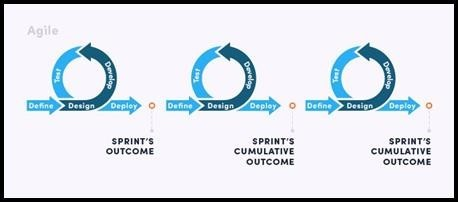
\includegraphics[scale=1.0]{Ch2/agile.jpg}

\label{fig:Prototype Model}

% Diagram change as per your project demands

\section{Scope of Proposed System}
Our experts found that the UI/UX of the old website was outdated and sluggish.During our research, we also found that the overall performance of the old website was slow due to several bugs and errors.\\
In the previous website, users could not add information regarding their personal portfolios and websites.Also, users were unable to share photos and reviews of purchased items on the website.



%\section{Hardware & Software Specifications}


% Write scope of your system.

\section{Technical Specification}
\textbullet \hspace{0.2cm} \textbf{Server}\\
Processor		:	Pentium 3\\
RAM          	: 	Min. 512 MB\\
Hard Disk		: 	Min. 480 MB free\\
\textbullet \hspace{0.2cm} \textbf{Client}\\
Processor   		: 	Pentium 3\\
RAM           	: 	Min. 512 MB\\
Hard Disk		: 	Min. 480 MB free\\
\textbullet \hspace{0.2cm} \textbf{Software Specification}\\
Platform	:  	Windows 10\\
Front End		: 	HTML, JavaScript, CSS.\\
Middle ware		: 	Python\\
Back End			: 	Expess.Js, Node.Js and MS-SQL \\	
Web Browser		: 	Chrome  101.0.4951.67  etc. \\


\subsection{ReactJs Framework}
The top tier of the MERN stack is React.js, the declarative JavaScript framework for creating dynamic client-side applications in HTML. React lets you build up complex interfaces through simple Components, connect them to data on your backend server, and render them as HTML. React is strong suit is handling stateful, data driven interfaces with minimal code and minimal pain, and it has all the bells and whistles you had expected from a modern web framework: great support for forms, error handling, events, lists, and more 
\\

\textbullet \hspace{0.2cm}	It underpins the Model/View/Controller (MVC) approach to web development—a best practice philosophy all developers should adhere to.\\

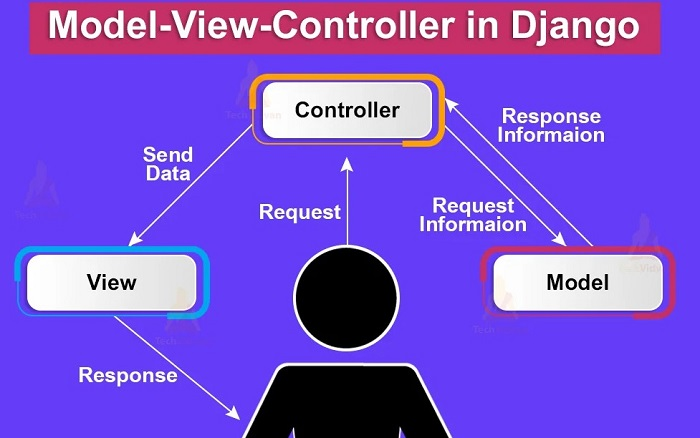
\includegraphics[scale=1.0]{Ch2/mvc1.jpg}


% Diagram change as per your project demands (If required)
\label{fig:MVC Model}

\subsection{Python}
\textbullet \hspace{0.2cm} Python becomes a wonderful choice when it comes to IoT. We can either use it for the backend side of development or the software development of devices. Moreover, Python is available to work on Linux devices, and we can make use of Micro Python for microcontrollers.  \\
\textbullet \hspace{0.2cm} Python is the coding language that we can use to reduce the volume of data that we need to deal with, accessible in the cloud. Python recognizes the needs regardless of whether we create the IoT project from scratch or interact with actuators, sensors, and accessories. \\  
\textbullet \hspace{0.2cm} Some of the many benefits of working with Python for IoT devices are a large number of libraries for all types of platforms and the speed it offers at which we can develop the code. 


%\textbullet \hspace{0.2cm}It’s built on a linear, easy-to-use folder structure.\\


% This section type your project contents 
\chapter{Feasibility Study}


\section{Introduction}
Therefore, a feasibility study of the proposed system needs to be carried out in order to:\\
\textbullet \hspace{0.2cm} 	Provide a better understanding of the System.\\
\textbullet \hspace{0.2cm}	Describe the outputs.\\

There are many factors. These factors are \textbf{Economical Feasibility, Technical Feasibility and Operational Feasibility}.\\

% This section type your project contents 


\section{Economical Feasibility}
\textbullet \hspace{0.2cm} This website is developed with the latest tools and technology which will full fill the client’s requirement.\\
\textbullet \hspace{0.2cm} Economic Feasibility helps in determining whether the required software has the potential to generate financial gains for an organization.\\
\textbullet \hspace{0.2cm} This type of study involves the cost incurred on the team of the software development, cost of study involved in conducting a feasibility study, estimated cost of software and hardware.\\
\textbullet \hspace{0.2cm} Here the cost of hardware is affordable.



% This section type your project contents 
\section{Operational Feasibility}
\textbullet \hspace{0.2cm} Further we can improve this website as per client’s needs.\\
\textbullet \hspace{0.2cm} Operational feasibility is studied to check, whether the human or employees in the business will use it or not. \\
\textbullet \hspace{0.2cm} Operational feasibility relies on human resources and analyses whether the software will operate after it is developed properly or not. \\
\textbullet \hspace{0.2cm} The GUI is designed to be user friendly, so it is easy to use by Users. 


\section{Technical Feasibility}
% This section type your project contents 
\textbullet \hspace{0.2cm} The user only requires Internet connection to use this website. So, this website is technically feasible. \\
\textbullet \hspace{0.2cm} Our system is technically feasible it is providing us required output.\\
\textbullet \hspace{0.2cm} The system is based on wireless technology and embedded system which are reasonably in phase with currently used technology. Therefore, it is very much favored by the technology.



\chapter{Proposed System}


\section{Proposed System}
Our main purpose is to create a Web application that make fastest-growing fashion influencing websites in which people sell their products with the help of other people. The remarkable thing about Bananoz is that your store will be promoted by hundreds of Bananoz's members.\\
\textbf{User/Influencers Registration:} 
 The first type of our system’s module is ‘User’. In our system, firstly User register into the system. After that User logged into the system. They can view products, reviews and feedbacks etc.\\
% This section type your project contents 


\textbf{Admin:}
The second type of system’s module is ‘ADMIN’. In our system, firstly Admin logged into system. After that Admin views all customer’s details, complaints, order details etc. Admin replies to customer’s complaints.\\
% This section type your project contents 



\section{User Privileges}

\begin{itemize}
\item Login
\item Registration
\item Promote Items
\item Upload Items
\item Search Products
\item Search Category
\item Search Users/Influencers
\item Place Order
\item Forget Password
\end{itemize}


% This section type your project contents 

\section{Objective of the System}
% This section type your project contents 

\begin{itemize}
\item Give Good Platform for Online Ecommerce
\item Latest technology 
\item Graphical user Interface
\end{itemize}
\chapter{Preliminary  Design}

\section{Tools of data flow strategy}
	Data flow strategy shows th and their interactions...........\\
\textbf{Data flow analysis makes use of the following tools:}\\
Flow Charts\\
Data Flow Diagrams\\
Data Dictionary\\
\textbf{Flowchart}\\
Flowchart is used to represent the algorithm .......\\
\textbf{Data Dictionary}\\
The logical characteristics of current systems data stores, including name, description, aliases, contents, ..........\\
\textbf{Data Structure Diagrams}\\
A pictorial description of the relation between entities (people, places, events and things) in system and the set of information about the entity, .........\\
\textbf{Structured Chart}\\
A design tool that pictorially shows the relation between processing modules in computer software, describes .............


%-----------------------------------------------------------------

\section{Use Case Diagram}
%If you add information about use case diagram\\
\subsubsection{Usecase Diagram For Admin}
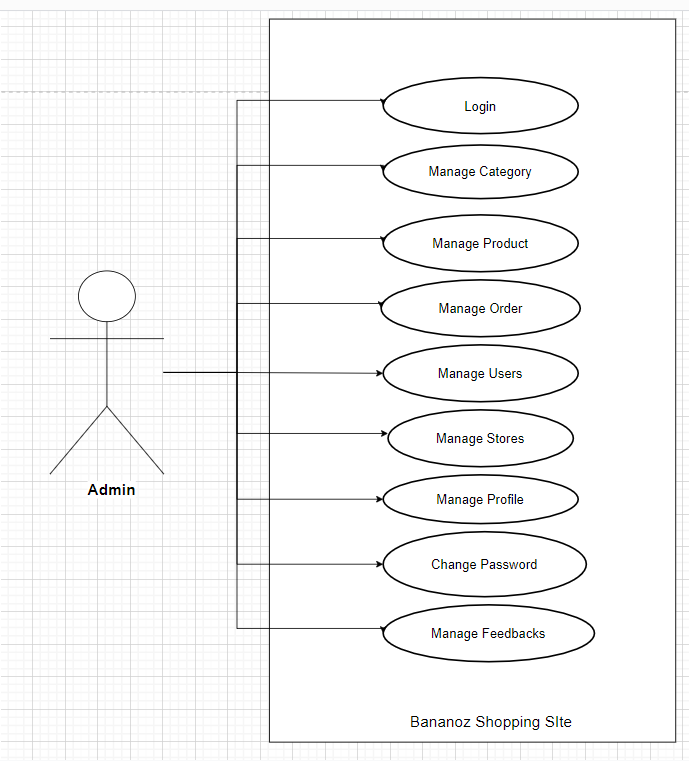
\includegraphics[scale=0.7]{Diag/admin-use-case.png}

\label{fig:Use case diagram For Admin}
\subsubsection{Usecase Diagram For Other Users.}
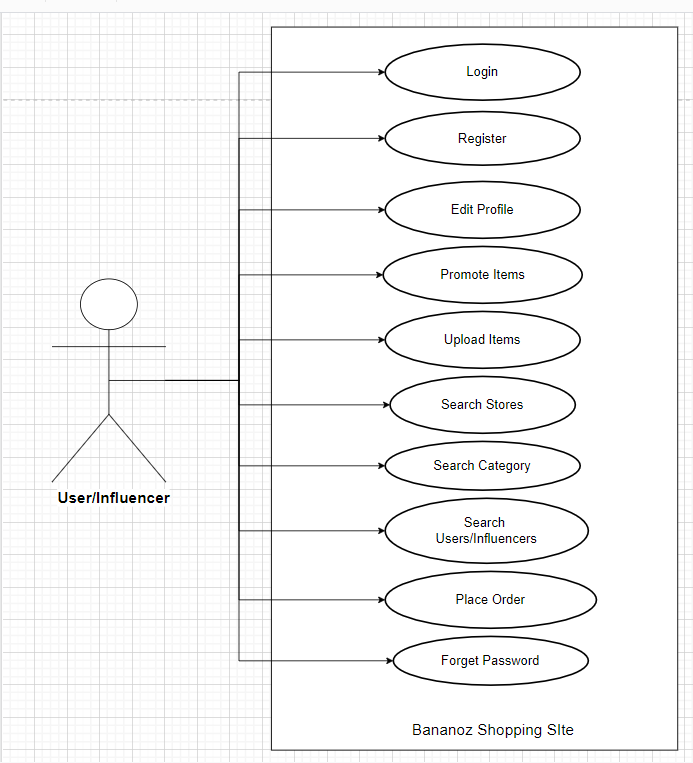
\includegraphics[scale=0.8]{Diag/user-use-case.png}

\label{fig:Use case diagram For User}



%-----------------------------------------------------------------
%\section{Activity Diagram}
%%If you add information about Activity Diagram\\
%
%\includegraphics[scale=.8]{Diag/activitylogin.png}
%\label{fig:Activity Diagram}



%-----------------------------------------------------------------

\section{Entity Relationship Diagram}

\subsubsection{ERD }
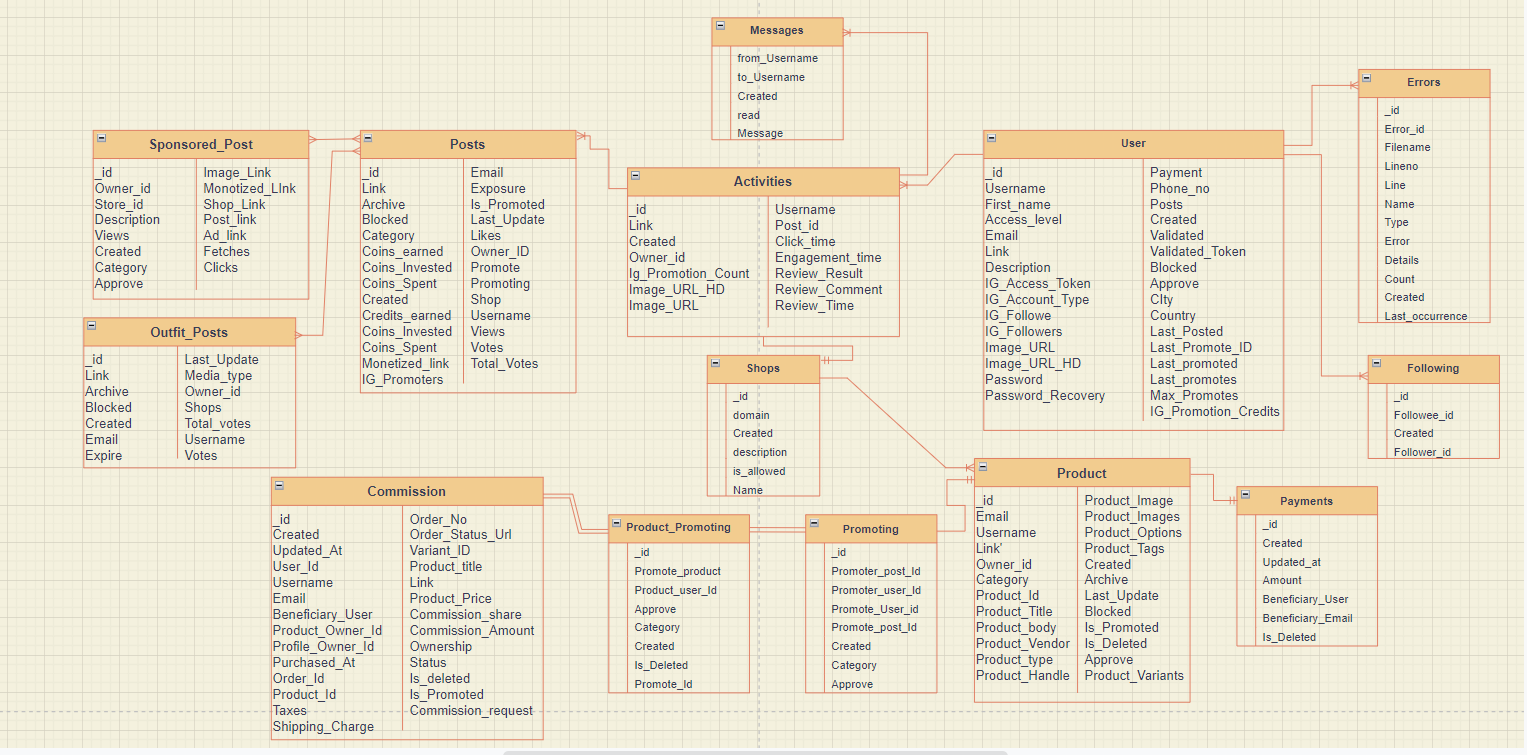
\includegraphics[scale=0.4]{Diag/database.png}
\label{abc}


%\subsubsection{ERD For users.}
%\includegraphics[scale=0.7]{Diag/ERDuser.png}
%\label{abc}
%
%\subsubsection{ERD For Products.}
%\includegraphics[scale=0.7]{Diag/ERDprod.png}
%\label{abc}
%-----------------------------------------------------------------

\section{Data Flow Diagram}
%If you add information about Data flow diagram\\

%\begin{figure} [h]
%\begin{center} 
\subsubsection{User Side Data Flow Diagram }
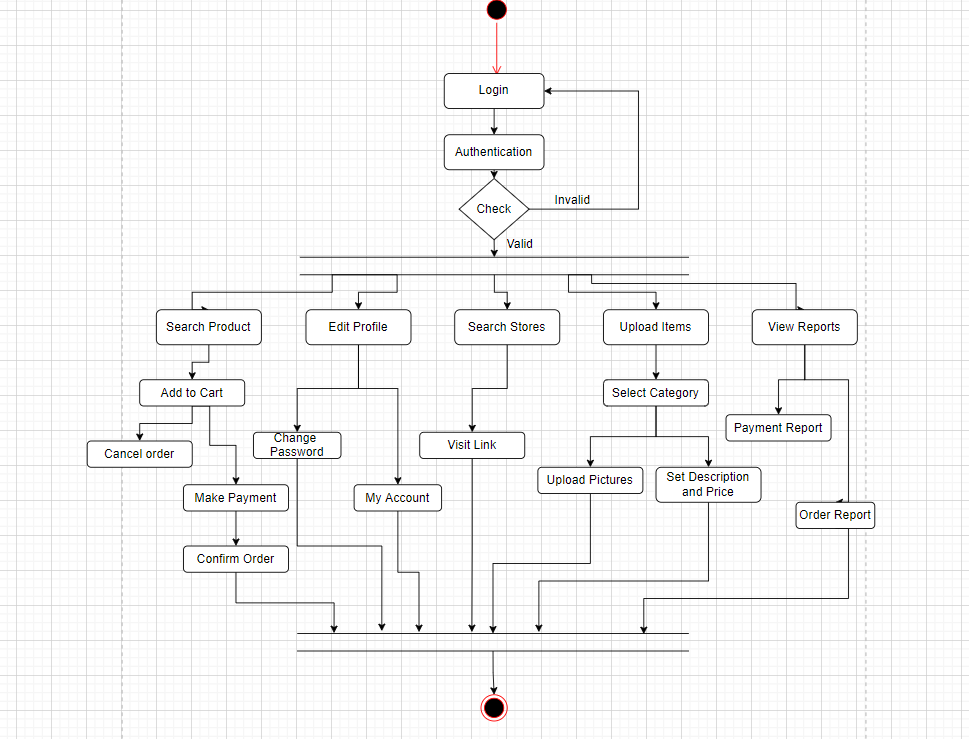
\includegraphics[scale = 0.6]{Diag/user-dfd.png}
\label{fig:Contex Level}


\subsubsection{Admin Side Data Flow Diagram }
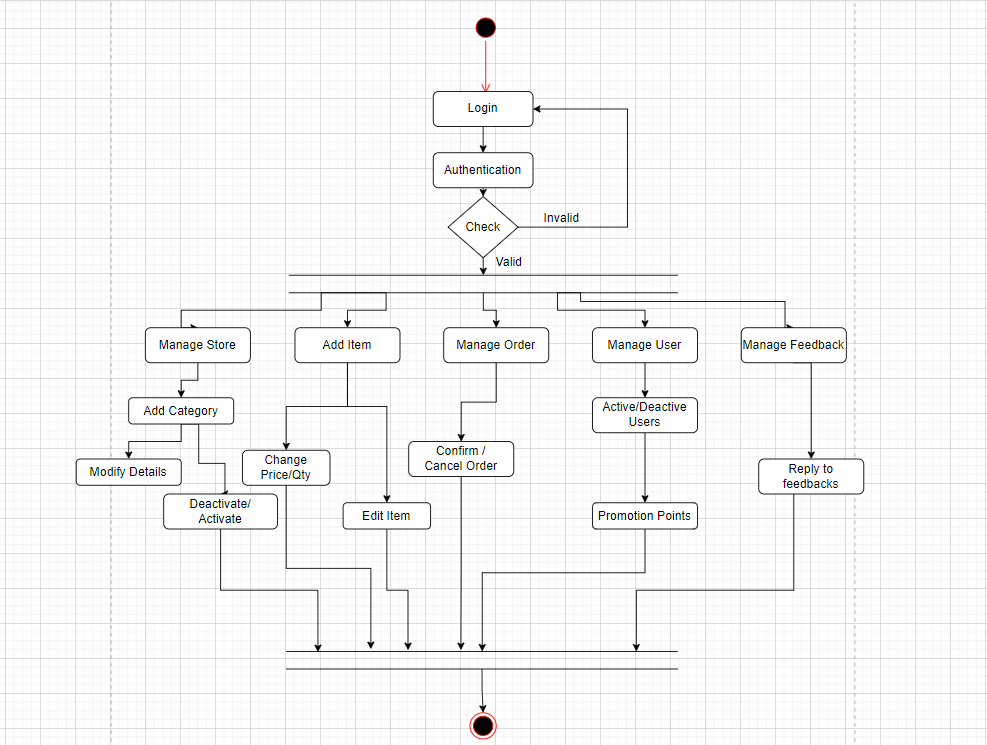
\includegraphics[scale=.8]{Diag/admin-dfd.png}
\label{fig:Contex Level}
%\end{center}
%\end{figure}



%\begin{figure} [h]
%\begin{center} 
%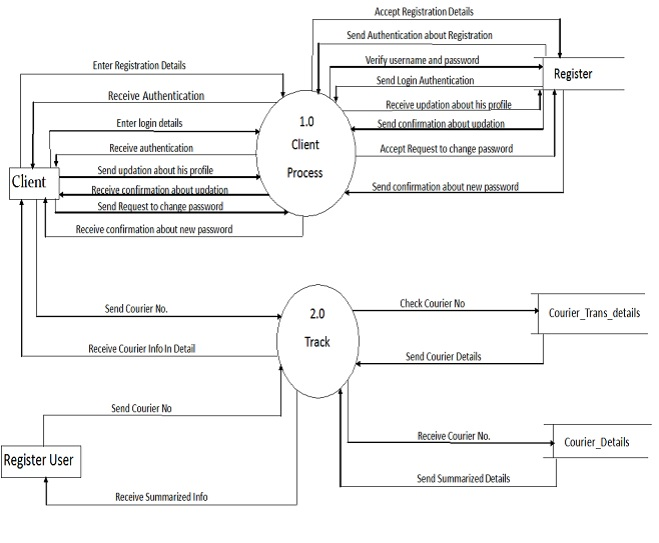
\includegraphics[scale=.9]{Ch5/dfd2.jpg}
%Fig. Data Flow Diagram
%\label{fig:DFD2}


\
% Students should divide chapter 3,4,5 according to major blocks of their project
\chapter{Testing Results}
\chapter{Conclusion and Future Scope}
\chapter{Concluding Remarks}


\section{Strengths of System}
\begin{enumerate}
\item 1.	System is easy to use....
\item 2.	System has a user friendly GUI...


\end{enumerate}
% This section type your project contents 

\section{Limitations of system}

\begin{itemize}
\item 1.	The only limitation of the system is that the system is not fully automated....
\item 2.	The limited scope of current System doesn’t fully encompass the current system.....


% This section type your project contents 
\end{itemize}

\section{Scope for future development} 

Our proposed solution is to revamp the website for client to stand out in competition.\\
Update it with new feature so that users can also upload photos of purchased items and write their honest reviews of the same.\\
We are going to add a feature in which influencers can add their personal website link to their Bananoz store.\\



% This section type your project contents 

\section{Conclusion}

\begin{itemize}
\item	The objective of this project was to develop a general-purpose e-commerce store where any product can be bought from the comfort of home through the Internet and to sell their products with the help of people from all over the world using famous social media “Instagram”. The website is to promote various products such as shirts, t-shirts, shoes, accessories, etc. for both men and women.\\


% This section type your project contents 

\item	Overall, my internship at KCS has been a success. I was able to gain practical skills, work in a fantastic environment, and make connections that will last a lifetime. I could not be more thankful.

\end{itemize}
%\addcontentsline{toc}{chapter}{References}


%\chapter*{Appendix}

%% Students are write appendix then write here., Otherwise Comment this chapter in chapter list (Select main.tex file and comment in front of appendix chapter)


\addcontentsline{toc}{chapter}{Appendix}
%\textbf{\centerline{Appendix}}	\\
\chapter*{\centerline{Appendix}}
\newpage
   % Not required then comment only 
\addcontentsline{toc}{chapter}{References}
\renewcommand\bibname{References}
\begin{thebibliography}{99}



% This section type your project contents 


\bibitem{Books} Websites,\\
Following websites proved to be very helpful during the development of the system.\\
•	https://www.academia.edu \\
•	https://logojoy.com \\
•	www.lucidchart.com \\ 
•	www.scribd.com \\
•	https://www.slideshare.net/ \\



% This section type your project contents 

\bibitem{diagrams} Software Used for Diagrams\\
•	Pacestar UML Diagrammer 6.\\
•	MS Vision 2010.\\


% This section type your project contents 
\end{thebibliography}
% ---------------------------------------------------------------------------------
% if any table wants to add in any chapter use following
%
%			\begin{table}[!ht]
%			\caption{Initial Testing Without Samples }   % name of table to be displayed above 						%											 				   table and in List of tables
%			\begin{tabular}{ c  c  c  c }				% table having 4 column
%							1 & 10 & 20 & 30 \\ 		% entries of column can separated by using &
%							2 & 40 & 50 & 60 \\ 		
%			\end{tabular}
%			\label{result1}		% for calling table no. in text
% 			\end{table} 
%
% ---------------------------------------------------------------------------------
\end{spacing}
\end{document}
